How much is a joker in the initial hand worth? We played $2{,}000$ \emph{mirror} games (both seats use the same strategy; seeds $50000$ and up) for random, max-tiles and joker-saver and grouped the $4{,}000$ initial hands per strategy by the number of jokers they contain (Table~\ref{tab:ini}, Figure~\ref{fig:ini}). Each entry is the mean score of hands with that number of jokers; the two hands of a game are counted separately and treated as independent in the intervals, an approximation we did not check.
\begin{table}[h]\centering\small
\caption{Mean score of an initial hand by number of jokers, mirror matches (95\% CI; number of hands in parentheses).}\label{tab:ini}
\begin{tabular}{@{}lccc@{}}\toprule
Strategy (mirror) & 0 jokers & 1 joker & 2 jokers\\\midrule
max-tiles & 0.497$\pm$0.018 (3025) & 0.507$\pm$0.033 (903) & 0.542$\pm$0.116 (72) \\
joker-saver & 0.466$\pm$0.018 (3025) & 0.600$\pm$0.031 (903) & 0.674$\pm$0.103 (72) \\
random & 0.504$\pm$0.018 (3025) & 0.494$\pm$0.033 (903) & 0.403$\pm$0.114 (72) \\
\bottomrule
\end{tabular}

\end{table}
\begin{figure}[h]\centering
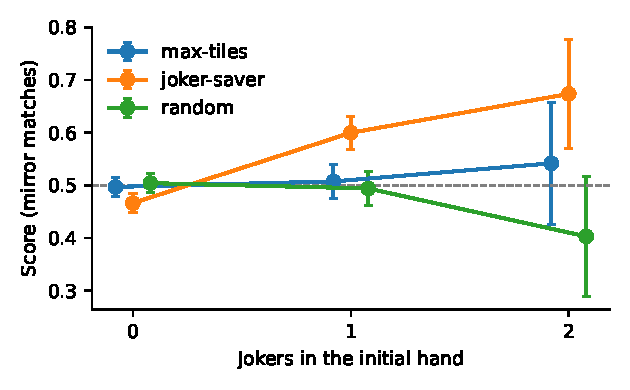
\includegraphics[width=0.5\linewidth]{figuras/coringas_iniciais.pdf}
\caption{Score by number of initial jokers, mirror matches.}\label{fig:ini}
\end{figure}
A joker in the opening hand is worth a substantial edge \emph{only for the joker-saver}: with one joker it scores $0.600\pm0.031$ and with two $0.674\pm0.103$ (72 hands only, so the interval is wide), against $0.466\pm0.018$ with none. Under max-tiles the score is $0.497$, $0.507\pm0.033$ and $0.542\pm0.116$, and under random $0.504$, $0.494\pm0.033$ and $0.403\pm0.114$, so a joker confers no detectable advantage to a player that does not hold it for the final move. This agrees with Section~\ref{sec:mech} (E4): the value of a joker depends on the policy that uses it. The two-joker estimate is imprecise and should not be read as a precise win probability.

\paragraph{Pooled field.} The mirror design covers only three strategies. To ask the question without fixing the strategy, we played $4{,}000$ games ($2{,}000$ seeds $\times$ 2 seatings, seeds $90000$ and up, official tie-break) in which each seed assigns one of the $28$ pairings, with repetition, of the seven strategies, and pooled the $8{,}000$ hands. Intervals resample seeds. Table~\ref{tab:campo} gives the result. A hand without an initial joker scores $0.496\pm0.006$, with one $0.509\pm0.020$, with two $0.576\pm0.081$ ($118$ hands): averaged over the field, a starting joker is worth about one or two points, and the interval for one joker contains $0.5$. Comparing, within each strategy, hands with and without a starting joker gives $+0.025$ [$0.000$, $0.052$].

\paragraph{Jokers drawn from the pool.} A joker can also arrive by drawing. Each player chooses to draw $29.7$ times per game on average (draws after the pool is empty are passes), so most of the $78$-tile pool is drawn: $50\%$ of hands ($3{,}991$ of $8{,}000$) draw at least one joker ($0.59$ per hand). A naive comparison is misleading: hands that drew a joker score $-0.015$ [$-0.043$, $0.012$] relative to those that did not, because players who draw more are usually behind and, drawing more, meet more jokers. We therefore compare hands within strata of the number of draws (five groups cut at the quintiles $23$, $27$, $31$, $38$; the pooled estimate uses strategy $\times$ quintile cells, the per-strategy estimates use the quintiles within each strategy), averaging the stratum differences with weights $n_1n_0/(n_1+n_0)$. The adjusted difference is $+0.037$ [$0.012$, $0.064$]. Figure~\ref{fig:comprado} shows the estimate per strategy: only the joker-saver has a clearly positive effect ($+0.119$ [$0.055$, $0.186$]), followed by max-points ($+0.081$ [$0.017$, $0.151$]) and max-tiles ($+0.053$ [$-0.015$, $0.120$]); random, cautious, min-play and no-rearrange are indistinguishable from zero. The joker-saver's drawn-joker effect agrees with its mirror-match initial-joker effect ($+0.13$). In the pooled field, however, the joker-saver's \emph{initial}-joker difference is $0.003$ ($0.681\pm0.066$ with one or more, $0.678\pm0.030$ with none; $251$ hands), about three standard errors below the mirror estimate; we did not find a reason, and note it as an open point (the opponent in the mirror also saves jokers for the last move, which may matter).
\begin{table}[h]\centering\small
\caption{Pooled field (seven strategies, $8{,}000$ hands): mean score by number of initial and drawn jokers, and effect of having a joker (hands with $\ge1$ minus hands with none). Intervals: normal over seeds for the group means; bootstrap over seeds for the effects. Bracketed values are 95\% intervals.}\label{tab:campo}
\begin{tabular}{@{}lcr@{}}\toprule
Group & Score (pooled field) & Hands\\\midrule
Initial jokers = 0 & 0.496$\pm$0.006 & 6068 \\
Initial jokers = 1 & 0.509$\pm$0.020 & 1814 \\
Initial jokers = 2 & 0.576$\pm$0.081 & 118 \\
\midrule
Bought jokers = 0 & 0.508$\pm$0.014 & 4009 \\
Bought jokers = 1 & 0.498$\pm$0.015 & 3282 \\
Bought jokers = 2 & 0.468$\pm$0.042 & 709 \\
\midrule
Initial joker, effect (strategy-stratified) & \multicolumn{2}{c}{$+0.025$ [+0.000, +0.052]} \\
Bought joker, naive difference & \multicolumn{2}{c}{$-0.015$ [-0.043, +0.011]} \\
Bought joker, stratified by draws & \multicolumn{2}{c}{$+0.037$ [+0.012, +0.064]} \\
\bottomrule
\end{tabular}

\end{table}
\begin{figure}[h]\centering
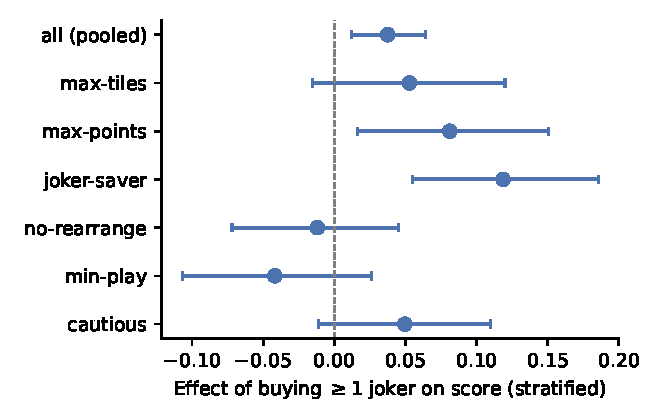
\includegraphics[width=0.55\linewidth]{figuras/coringa_comprado.pdf}
\caption{Effect of drawing at least one joker on the score, within strata of the number of draws, by strategy (95\% bootstrap intervals).}\label{fig:comprado}
\end{figure}
Both routes lead to the same conclusion as Section~\ref{sec:mech}: a joker is worth little to a player who spends it as soon as it helps, and its value is realised by the strategy that holds it for the last move. Because the player cannot choose when a joker arrives, this is a statement about the policy, not about the tile.
